\chapter{Introduction}
\label{chp:intro}
\noindent In this Chapter, introduction of \gls{webrtc} and \gls{sip} network will be covered. \gls{sip} is one of the \gls{voip} signaling protocols widely used in current internet telephony service which is the target telephony network integrated with \gls{webrtc} application system in this thesis.

\section{WebRTC}

\noindent Gmail\footnote{Gmail is a free , advertising-supported email service provided by Google.} video chat became popular in 2008, and in 2011 Google introduced Hangouts\footnote{Google Hangouts is an instant messaging and video chat platform developed by Google, which launched on May 15, 2013 during the keynote of its I/O development conference. It replaces three messaging products that Google had implemented concurrently within its services, including Talk, Google+ Messenger, and Hangouts, a video chat system present within Google+.}, which use the Google Talk service (as does Gmail). Google bought \gls{gips}, a company which had developed many components required for \gls{rtc}, such as codecs and echo cancellation techniques. Google open sourced the technologies developed by \gls{gips} and engaged with relevant standards bodies at the \gls{ietf} and \gls{w3c} to ensure industry consensus. In May 2011, Ericsson built the first implementation of \gls{webrtc}.

\subsection{What is WebRTC ?}

\noindent \gls{webrtc} is an industry and standards effort to put real-time communications capabilities into all browsers and make these capabilities accessible to web developers via standard \gls{html5} tags and JavaScript \gls{api}s. For example, consider functionality similar to that offered by Skype\footnote{Skype is a freemium voice-over-IP service and instant messaging client, currently developed by the Microsoft Skype Division.\cite{wiki:skype}}. but without having to install any software or plug-ins. For a website or web application to work regardless of which browser is used, standards are required. Also, standards are required so that browsers can communicate with non-browsers, including enterprise and service provider telephony and communications equipment\cite{inbook:rtc-intro}.

\par With the rapidly development of internet, more and more communication traffic is moving to web from the traditional telephony network. And in the recent decade, \gls{voip} network services are growing to the peek of the market capacity. Solution to integrate \gls{webrtc} and existing \gls{voip} network is the right approach the trend of the internet communication requirement.

\subsection{WebRTC Network Structure}
\noindent In the Figure\ref{fig:webrtc_network_finCandidate}\cite{html5rock:webrtc} showing how the \gls{ice} framework\footnote{ICE is a framework for connecting peers, such as two video chat clients.\cite{wiki:ice}} to find peer candidate through \gls{stun} server and its extension \gls{turn} server. The difference and usage of \gls{stun} server and \gls{turn} server will be discussed more detail in Chapter \ref{chp:sys_deploy}.
\par \gls{webrtc} needs server to help users discover each other and exchange 'real world' details such as names. Then \gls{webrtc} client applications (peers) exchange network information. After that, peers exchange data about media such as video format and resolution. Finally, \gls{webrtc} client applications can traverse \gls{nat} gateways and firewalls.

\begin{figure}
	\centering
    	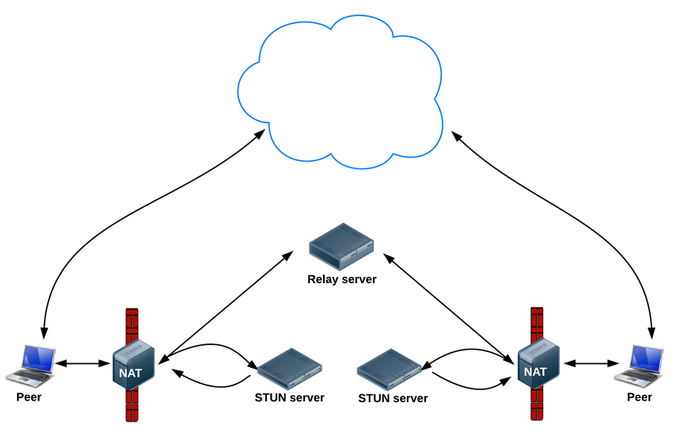
\includegraphics[height=0.30\textheight,natwidth=610,natheight=642]{figs/webrtc_network_finCandidate.png}
  	\caption{\gls{webrtc} Network: Finding connection candidates}
  	\label{fig:webrtc_network_finCandidate}
\end{figure} 

\begin{figure}
	\centering
    	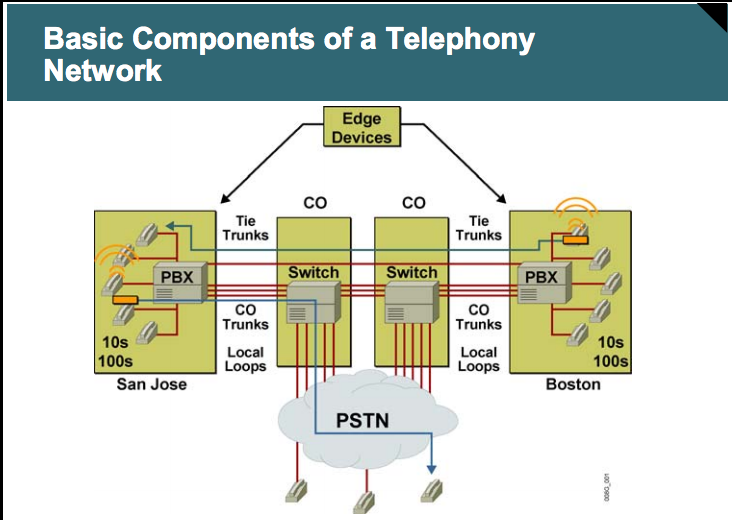
\includegraphics[height=0.40\textheight,natwidth=610,natheight=642]{figs/telephony_network.png}
  	\caption{Traditional Telephony Network}
  	\label{fig:telephony_network}
\end{figure}

\par Compare to the traditional telephony network which is shown in Figure\ref{fig:telephony_network}\cite{web:teleVSvoip}, the main difference between these two communication network is that \gls{webrtc} is \gls{p2p} communication, in \gls{stun} server scenario, after the signaling between end-peers, the media data are exchanged directly between tow peers, but in the traditional telephony, all the media data are transferred to \gls{pbx} and switches regarding to \gls{pstn}\footnote{The PSTN consists of telephone lines, fiber optic cables, microwave transmission links, cellular networks, communications satellites, and undersea telephone cables, all interconnected by switching centers, thus allowing any telephone in the world to communicate with any other. Originally a network of fixed-line analog telephone systems, the PSTN is now almost entirely digital in its core network and includes mobile and other networks, as well as fixed telephones.\cite{wiki:pstn}} then reach the other side of the peer. Even in \gls{turn} server scenario, the media stream is only relaying to the \gls{turn} then directly transfer to another peer, no switches involved.

\subsection{WebRTC Implementation APIs}

\begin{figure}
	\centering
    	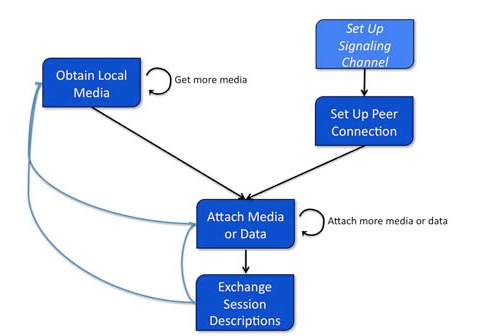
\includegraphics[width=0.50\textheight,natwidth=610,natheight=642]{figs/webrtcApis.png}
  	\caption{WebRTC \gls{api} View with Signaling\cite{inbook:rtc-apis}}
  	\label{fig:webrtc_4steps}
\end{figure}

\noindent There are four main steps to implement a \gls{webrtc} session. The Figure \ref{fig:webrtc_4steps} shows that the browser client need to obtain local media first, then set up a connection between the browser and the other peer through some signaling, after that attach the media and data channels to the connection, afterwards exchange the session description from each other. Finally the media stream will automatically exchange through the real-time peer to peer media channel.

\par In order to obtain local media, the \gls{webrtc} \gls{api}s provide \textit{getUserMedia()} function to get the video and audio stream from user. For privacy reasons, a web application’s request for access to a user’s microphone or camera will only be granted after the browser has obtained permission from the user. \textit{getUserMedia()} function is currently available in Chrome, Opera and Firefox. Almost all of the \gls{webrtc} \gls{api}s are slightly different in different browsers, then this part will be discussed in the Chapter \ref{chp:sys_dev}. However, since \gls{webrtc} \gls{api}s is not standard \gls{api} yet, the prototype application in this thesis will not pay too much work-load on compatibility for different browsers platform.

\par For setting up peer connection, the core of \gls{webrtc} is the \textit{RTCPeerConnection} \gls{api}, which sets up a connection between two peers. In this context, “peers” means two communication endpoints on the World Wide Web. Instead of requiring communication through a server, the communication is direct between the two entities. In the specific case of \gls{webrtc}, a peer connection is a direct media connection between two web browsers. This is particularly relevant when a multi-way communication such as a conference call is set up among three or more browsers. Each pair of browsers will require a single peer connection to join them, allowing for audio and video media to flow directly between the two peers. The system architecture regarding to this \gls{webrtc} factor will be discussed in later Chapter \ref{chp:sys_dev} since there is consideration between centralized media server network and mesh network architecture.

\begin{figure}
	\centering
    	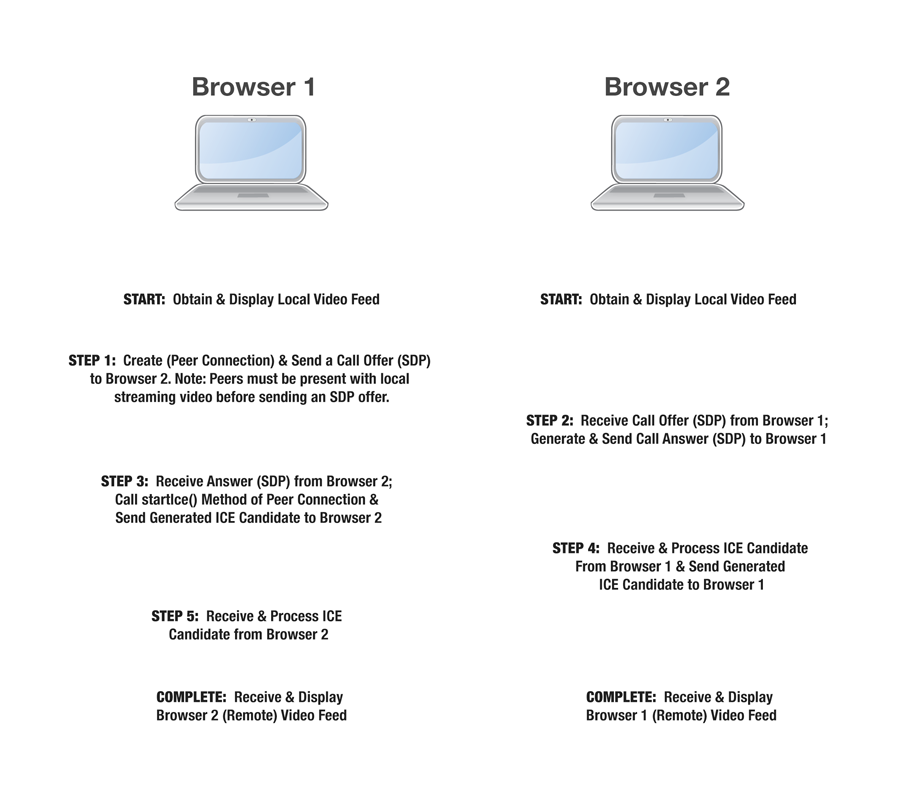
\includegraphics[width=0.60\textheight,natwidth=610,natheight=642]{figs/webrtc_diagram.png}
  	\caption{WebRTC Set up a call Process}
  	\label{fig:webrtc_diagram}
\end{figure}

\par To establish this connection requires a new \textit{RTCPeerConnection} object. The only input to the \textit{RTCPeerConnection} constructor method is a configuration object containing the information that \gls{ice}, will use to “punch holes” through intervening \gls{nat} devices and firewalls. There are two \gls{api}s to handle the  \textit{IceCandidate} object which contains \gls{ice} information data. One is \textit{onicecandidate} listener to trigger the function to handle the new \textit{IceCandidate} data object. The other one is \textit{addIceCandidate} function to add the new \textit{IceCandidate} data object to the remote/local peer connection session description field.

\par \gls{ice} is a framework for connecting peers, such as two video chat clients. Initially, \gls{ice} tries to connect peers directly, with the lowest possible latency, via \gls{udp}. In this process, \gls{stun} servers have a single task: to enable a peer behind a \gls{nat} to find out its public address and port. If \gls{udp} fails, \gls{ice} tries \gls{tcp}: first \gls{http}, then \gls{https}. If direct connection fails—in particular, because of enterprise \gls{nat} traversal and firewalls—\gls{ice} uses an intermediary (relay) \gls{turn} server. In other words, \gls{ice} will first use \gls{stun} with \gls{udp} to directly connect peers and, if that fails, will fall back to a \gls{turn} relay server. The expression 'finding candidates' refers to the process of finding network interfaces and ports.\cite{html5rock:webrtc} 

\par Once the \textit{RTCPeerConnection} is established, the client need configure where the media or data to store and display if it is necessary. In the prototype application of this thesis, media stream will be displayed in a \gls{html5} tag called \textit{<video>}. It will only be shown when there is media stream in \textit{<video>} tag source.

\par In order to make the \gls{webrtc} \gls{stun} server or \gls{turn} server to generate the \gls{ice} candidate for the peer client, the caller \textit{RTCPeerConnection} need run \textit{createOffer()} function and the callee need run \textit{createAnswer()} function  to ask the \gls{stun}/\gls{turn} server to find the path for each other peer.There is one calling process shown in Figure\ref{fig:webrtc_diagram}, it is a set up call process from caller peer.

\par \gls{webrtc} clients (known as peers) also need to ascertain and exchange local and remote audio and video media information, such as resolution and codec capabilities. Signaling to exchange media configuration information proceeds by exchanging an offer and an answer using the \gls{sdp}. The \textit{createOffer()} function and \textit{createAnswer()} function both have callback function to handle the \gls{sdp} either to call \textit{setLocalDescription()} by caller or call \textit{setRemoteDescription()} by callee when callee gets the caller's \gls{sdp} from \gls{webrtc} offer. The Log Snippet\ref{log:webrtc_answer_sdp} shown is the \gls{webrtc} answer \gls{sdp} from the callee when the callee end-point decide to accept this conversion session.

\begin{algorithm}[h]
\floatname{algorithm}{Log Snippet}
  \caption{Sample \gls{webrtc} Answer \gls{sdp}}
  \label{log:webrtc_answer_sdp}
  \begin{verbatim}
sdp: v=0
o=xmserver 1399363527 1399363528 IN IP4 10.254.9.135
s=xmserver
c=IN IP4 10.254.9.135
t=0 0
a=ice-lite
m=audio 49152 RTP/SAVPF 0 126
a=rtpmap:0 PCMU/8000
a=sendrecv
a=rtcp:49153
a=candidate:1 1 UDP 2130706431 10.254.9.135 49152 typ host
a=candidate:1 2 UDP 2130706430 10.254.9.135 49153 typ host
...
a=acfg:1 t=1
a=rtpmap:126 telephone-event/8000
a=fmtp:126 0-15
m=video 57344 RTP/SAVPF 100
b=AS:1000
a=rtpmap:100 VP8/90000
a=fmtp:100 max-fr=30; max-fs=1200
a=sendrecv
a=rtcp:57345
a=rtcp-fb:100 ccm fir
a=rtcp-fb:100 nack
a=rtcp-fb:100 nack pli
a=rtcp-fb:100 goog-remb
a=candidate:2 1 UDP 2130706431 10.254.9.135 57344 typ host
a=candidate:2 2 UDP 2130706430 10.254.9.135 57345 typ host
...
 \end{verbatim}
\end{algorithm}

\section{SIP Network}